\chapter{Results}

I have tested the two algorithms described in \nameref{chap:design} using the structure given in \nameref{chap:implementation}.\\
There are two major parts which should be analyzed: the correctness of the algorithm and it's running time.

\section{Correctness}

We have collected a set of $4500$ images from the Internet, which we have classified in about $1600$ similarity sets, each set being composed of up to five images. The images within a similarity set differ in size, having various watermarks and filters applied (these sets are known to be correct beforehand). We have inserted these images in a larger set of $100.000$ images taken from the Internet and performed a queries for each of the $4500$ images of the similarity sets, getting the top $10$ similar images. We want to observe:
\begin{itemize}
	\item if the algorithm finds the exact match, i.e. the image that has been queried with
	\item if the algorithm finds the other images which are part of the same similarity set
	\item the mean running time of a query
	\item how varying the metrics described above influences the results of the query
\end{itemize}

We evaluate the response to a query, by looking at the indices of the images from the current similarity set in the list of results returned by the query. Thus, the $index\ score$ for a certain query can be computed as the sum of these indices; the smaller the sum, the closer in the response list are the images we want to find. \\
For the set of $100.000$ images we use $P=20$ KD-trees, each KD-tree storing the descriptors for $N=5000$ images.\\
The results of this test can be seen in the following two tables. The first one describes, for similarity sets of size $3$, $4$ and $5$, and for the metrics described in \nameref{section:algorithm}, the average number of how many of these images are found in the list of $10$ returned images.\\

\begin{center}
\begin{tabular} {c | c | c | c}
	& max nr descs & min avg & max dist to avg \\
	\hline
	3 & 2.47 & 2.37 & 2.52 \\
	\hline
	4 & 3.26 & 3.21 & 3.38 \\
	\hline
	5 & 3.98 & 3.63 & 4.14 \\
\end{tabular}
\end{center}

The second table shows the $index\ score$ (described above) for the same queries and metrics.\\

\begin{center}
\begin{tabular} {c | c | c | c}
	& max nr descs & min avg & max dist to avg \\
	\hline
	3 & 8.32 & 9.29 & 7.84 \\
	\hline
	4 & 12.69 & 13.15 & 11.76 \\
	\hline
	5 & 18.35 & 21.36 & 17.10 \\
\end{tabular}
\end{center}

It can be observed that the third metric, the largest distance from the descriptors of an image to the average of all found descriptors, provides the best results.\\

Also, we have constructed a single KD-tree which contains the $4500$ images from the similarity set in order to test the three different metrics described in \nameref{section:algorithm} for selecting the filtered images.\\
We retained the $image\ pair\ score$ of the returned similar images, and evaluated these three metrics by computing the following $correctness\ scores$:
\begin{itemize}
	\item the mean between the $image\ pair\ scores$
	\item the sum of the differences between the $pair\ scores$ of two consecutive similar images in the returned list
	\item the maximum $image\ pair\ score$
\end{itemize}
The goal is to minimize each of these $correctness\ scores$.

The results of this test are shown in the next table:\\
\\
\begin{center}
\begin{tabular} {c | c | c | c}
	& max nr descs & min avg & max dist to avg \\
	\hline
	mean & 661880 & 693745 & 647355 \\
	\hline
	sum of diff & 867877 & 1021543 & 856521 \\
	\hline
	max score & 1162618 & 1134470 & 1150899 \\
\end{tabular}
\end{center}

As it can be seen, the third metric, largest distance from the descriptors of an image to the average of all found descriptors, performs the best out of the three metrics.

\section{Running Time}
We have tested our algorithm on a machine with 55GB of RAM, 16 quad-core processors with a frequency of 2.4GHz.\\

The first experiment that we did was comparing the runtimes of the $linear\ algorithm$ with the $kdtree\ algorithm$ by running them on sets of $5, 10, 20, 50, 200, 350$ and $500$ images. The corresponding running times are shown in Figure~\ref{fig:runtimesBasic}.\\
The red line shows the corresponding running times for the $linear\ algorithm$, while the green one shows the times for the $kdtree\ algorithm$. As it can be seen, the $kdtree\ algorithm$ outperformes the linear one, with the same returned image (so it does not give different results). The non-ascending running times of the $kdtree\ algorithm$ can be explained by the fact that the KD-tree data structure is traversed heuristically, so depending on the given input a certain query can execute with varying running times. For a KD-tree of $5000$ images and $5000$ queries, the mean running time of a search is $1.36$ seconds.\\
Of course, the $kdtree\ algorithm$ does require an initialization time, which is the price that has to be paid in order to perform fast queries. Figure~\ref{fig:totalRuntimes} shows the sum between the initialization time and query time of a linear image server and an image server which constructs a KD-tree. As it can be seen, the initialization time for the KD-tree grows linearly, but this gets compensated by the small query time. For a $500$-size image set, the initialization and a query on the KD-tree takes $36.771$ seconds, which is less than a query on the same image set using the $linear\ algorithm$, which takes $77.331$ seconds.

\begin{figure}[ht!]
\centering
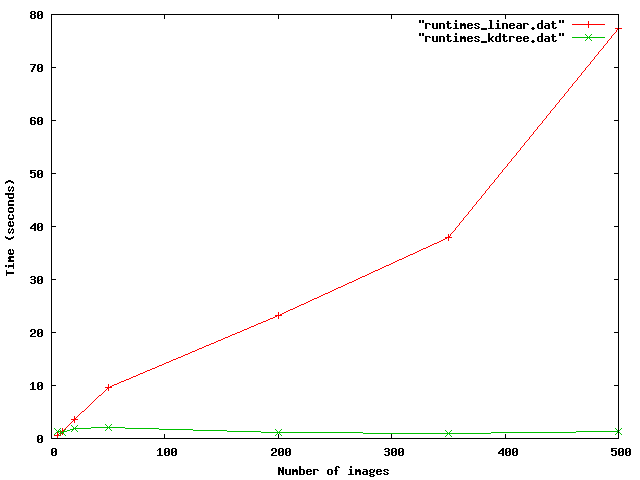
\includegraphics[width=.7\linewidth]{images/runtimesBasic.png}
\caption{Runtime of the two algorithms}
\label{fig:runtimesBasic}
\end{figure}

\begin{figure}[ht!]
\centering
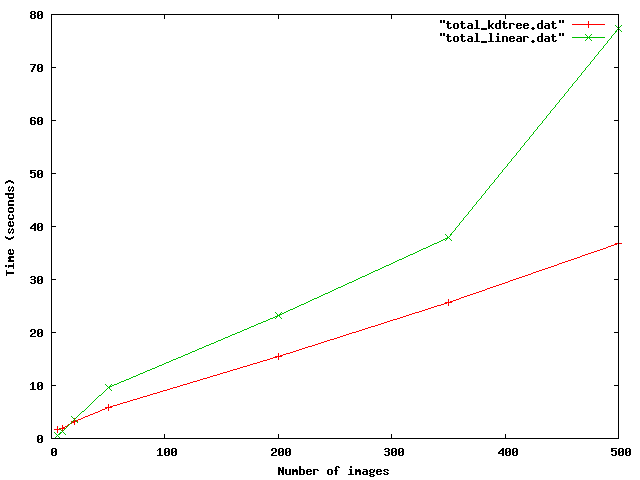
\includegraphics[width=.7\linewidth]{images/totalRuntimes.png}
\caption{Total query time for $linear\ algorithm$ and $kdtree\ algorithm$}
\label{fig:totalRuntimes}
\end{figure}

The second set of tests have been concentrated on analyzing the behavior of large scale KD-trees.
As stated above, our main concern was the initialization time of a KD-tree, which is divided into two steps: the computation of the descriptors for the images, and the construction of the actual KD-tree.\\
In Figure~\ref{fig:totalInit} we can see the total initialization time for a KD-tree, and the time needed only for the construction of the KD-tree data structure (presuming that the descriptors are already computed). \\
\begin{figure}[ht!]
\centering
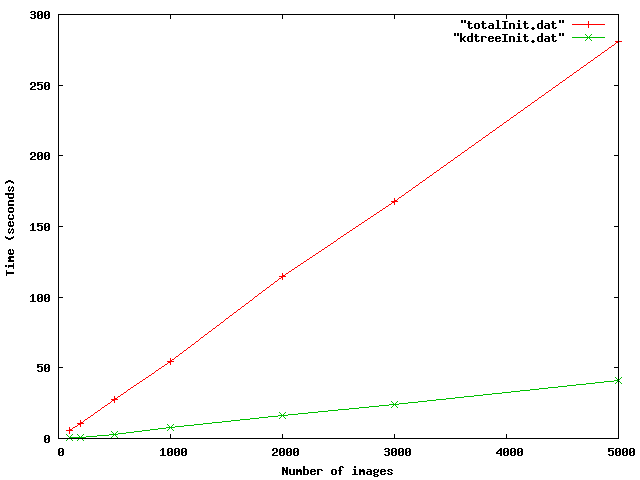
\includegraphics[width=.8\linewidth]{images/totalInit.png}
\caption{Initialization runtimes}
\label{fig:totalInit}
\end{figure}

\begin{center}
\begin{tabular} {c | c | c}
	number of images & total init (seconds) & kdtree init (seconds) \\
	\hline
	100 & 5.34 & 0.48 \\
	200 & 10.53 & 0.99 \\
	500 & 27.71 & 3.17 \\
	1000 & 54.52 & 7.72 \\
	2000 & 114.27 & 16.26 \\
	3000 & 167.83 & 24.31 \\
	5000 & 280.67 & 41.20 \\
\end{tabular}
\end{center}

Because the total number of images is divided into KD-trees of fixed dimension (in our case $5000$ images), inserting a new image into our database is constant, because it just implies creating a new KD-tree (or expanding a current one, if its dimension doesn't exceed $5000$ images).
